% Chapter Template

\chapter{Valgrind} % Main chapter title

\label{Chapitre 4.1} % Change X to a consecutive number; for referencing this chapter elsewhere, use \ref{ChapterX}

\lhead{ \emph{Valgrind}} % Change X to a consecutive number; this is for the header on each page - perhaps a shortened title

%----------------------------------------------------------------------------------------
%	SECTION 1
%----------------------------------------------------------------------------------------


\section{Runtime memory analysis and vulnerability detection}
Les deux codes fournis comportent des erreurs de fonctionnement qu'il va falloir découvrir et corriger. Ces codes ont une syntaxe correcte et sont compilables, ce qui ne veut pas dire qu'ils sont corrects et il faut notamment vérifier la manière dont il gèrent la mémoire allouée dynamiquement (allocation, libération, accès) car des erreurs à ce niveau ne sont pas visibles lors de la compilation.\\
Pour les découvrir, on utilise les outils Valgrind vu au cours : "memcheck", "sgcheck" et "massif".

\subsection{Code 1 : bitmap.c}
Ce premier code encode une image dans une autre par stéganographie. Pour ce faire il copie les images dans une zone mémoire allouée dynamiquement, et quand il a terminé il libère cette zone mémoire.\\

On va d'abord voir si sa mémoire est bien gérée ou non avec l'outil massif :
\begin{lstlisting}[frame=single,style=Console]  % Start your code-block

valgrind --tool=massif --time-unit=B ./bitmap
\end{lstlisting}

\begin{center} 
\hspace{15cm}
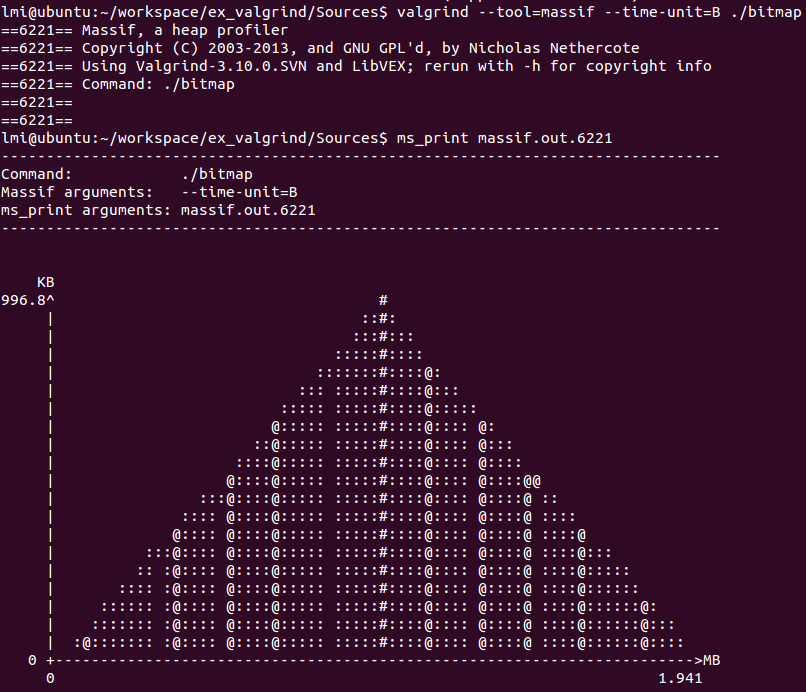
\includegraphics[width=8cm]{massif_avant_modif.png}
\end{center}
\vspace{0.5cm}
Dans ce cas là on ne voit pas grand chose... Si ce n'est que la quantité de mémoire utilisée à la fin du programme est libérée (ou presque, peut-être quelques octets nous échappent, avec une échelle qui va jusqu'à 1MB on ne voit pas une différence de quelques octets...)\\

On va donc essayer avec memcheck :
\begin{lstlisting}[frame=single,style=Console]  % Start your code-block

valgrind --tool=memcheck --leak-check=full ./bitmap
\end{lstlisting}
\begin{center} 
\hspace{15cm}
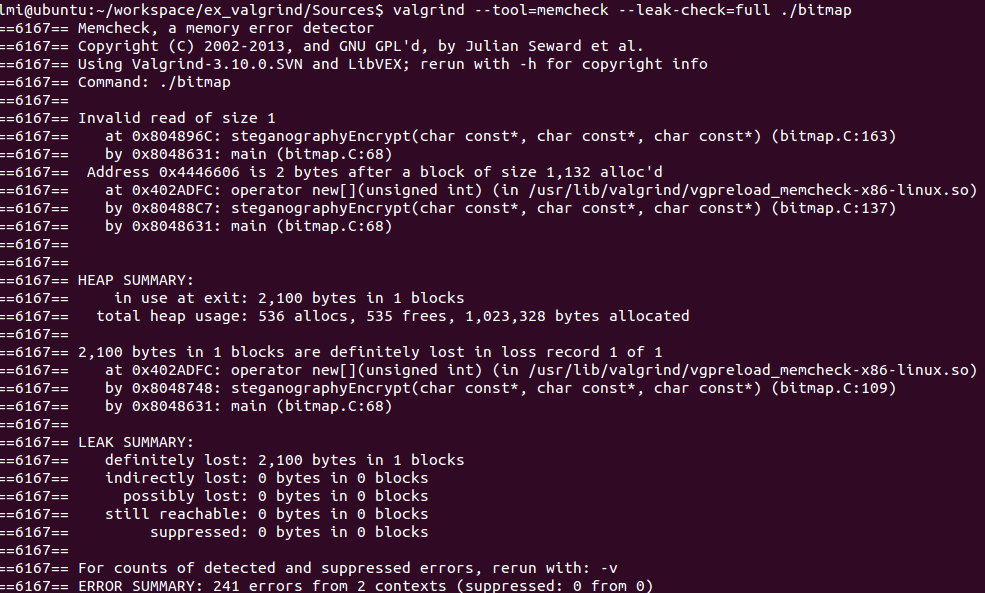
\includegraphics[width=8cm]{memcheck_avant_modif.png}
\end{center}
\vspace{0.5cm}
Cette fois on voit qu'il se passe des choses incorrectes durant l'exécution du programme. Notamment qu'à un moment il y a un accès mémoire 2 bytes plus loin que la fin d'un bloc alloué dynamiquement, ainsi que toute la mémoire n'est pas libérée à la fin (536 blocs alloués mais seulement 535 libérés, ce qui fait qu'un bloc de (d'une taille de 2.1kB) est définitivement perdu).\\

En cherchant un peu dans le code, on trouve assez facilement les deux erreurs.\\

La première est assez grossière et très visible. Elle mène à l'accès mémoire 2 bytes plus loin que la fin du bloc alloué. On voit ci-dessous (ligne 161 du fichier bitmap.c) qu'une boucle for itère jusqu'à un indice dépassant de 2 la largeur de l'image (+2 ajouté à l'indice), et donc accède à une zone mémoire dépassant la taille du bloc alloué.
\begin{center} 
\hspace{15cm}
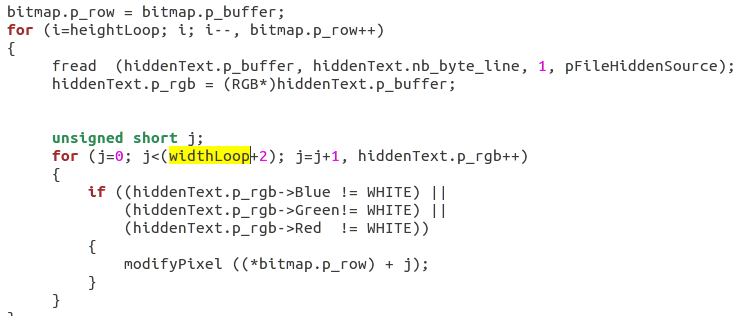
\includegraphics[width=14cm]{modif_code1.png}
\end{center}
\vspace{0.5cm}

La seconde est classique elle aussi, même si elle est moins visible. La zone mémoire allouée dynamiquement pour l'image est réservée sous la forme d'un tableau de tableaux (tableau 2D). Donc un premier tableau est alloué pour contenir tous les pointeurs vers les autres tableaux qui contiendront, eux, l'image elle-même. Seulement lors de la libération de la mémoire, les tableaux contenant l'image sont libérés, mais le tableau contenant les pointeurs est oublié, ce qui provoque la fuite mémoire.
\begin{center} 
\hspace{15cm}
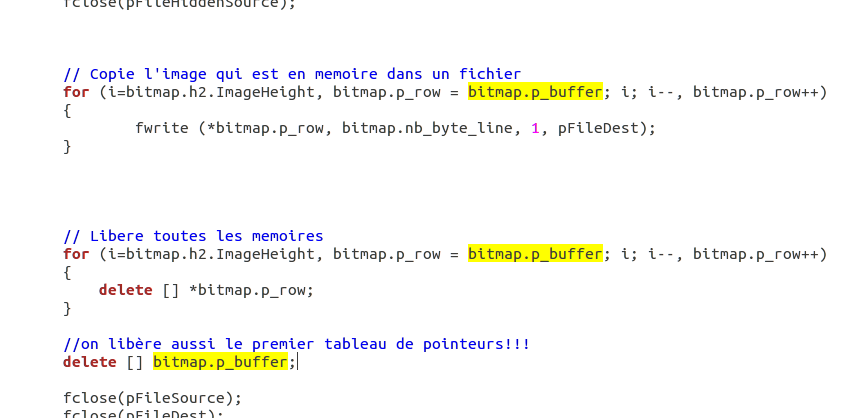
\includegraphics[width=14cm]{modif_code2.png}
\end{center}
\vspace{0.5cm}

Et maintenant si on relance la commande memcheck sur le code corrigé, elle ne trouve plus de problème lors de l'exécution du programme.
\begin{center} 
\hspace{15cm}
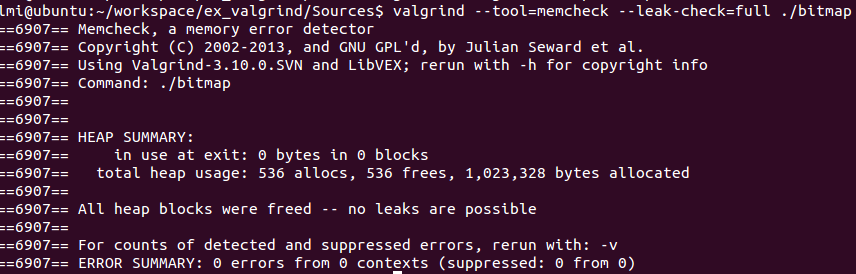
\includegraphics[width=14cm]{memcheck_apres_modifs.png}
\end{center}
\vspace{0.5cm}

L'outil sgcheck quant à lui n'a rien donné sur ce programme. Il n'a pas trouvé de problème car il est fait pour détecter des dépassement de pile ou de tableaux (mais pas sur l'allocation dynamique apparemment), et il n'y avait donc pas de problème détectable pour lui.\\

\pagebreak
\subsection{Code 2 : exe2.c}
Le second code est extrêmement mal écrit! Après une longue étude (:-P) du programme, il s'avère que c'est une implémentation de vecteurs en C. Si on compile le code et qu'on l'exécute avec les outils "Valgrind" pour tester les fuites mémoire, on obtient le résultat suivant :
\begin{center} 
\hspace{15cm}
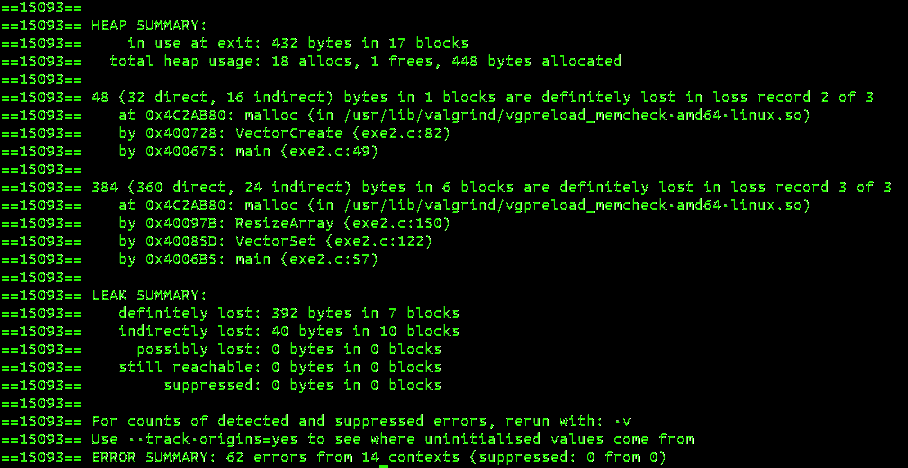
\includegraphics[width=14cm]{memcheck_avant_exe2.png}
\end{center}
\vspace{0.5cm}

On remarque que 392 bytes ont étés perdus après allocations. Si on utilise l'outil massif on voit clairement que rien n'est libéré :
\begin{lstlisting}[frame=single,style=Console]  % Start your code-block

valgrind --tool=massif --time-unit=B ./exe2_orig
\end{lstlisting}
\begin{center} 
\hspace{15cm}
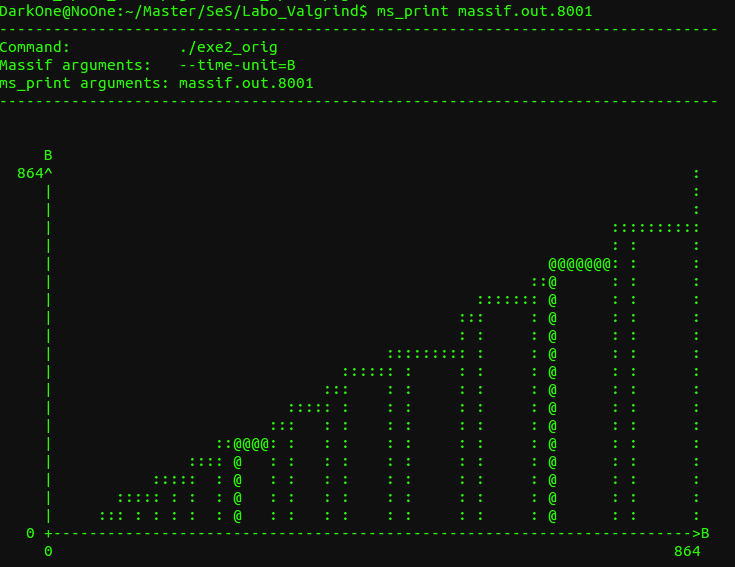
\includegraphics[width=14cm]{massif_exe2_avant.png}
\end{center}
\vspace{0.5cm}
\pagebreak





Commençons par la modification de la fonction "main" :
\begin{center} 
\hspace{15cm}
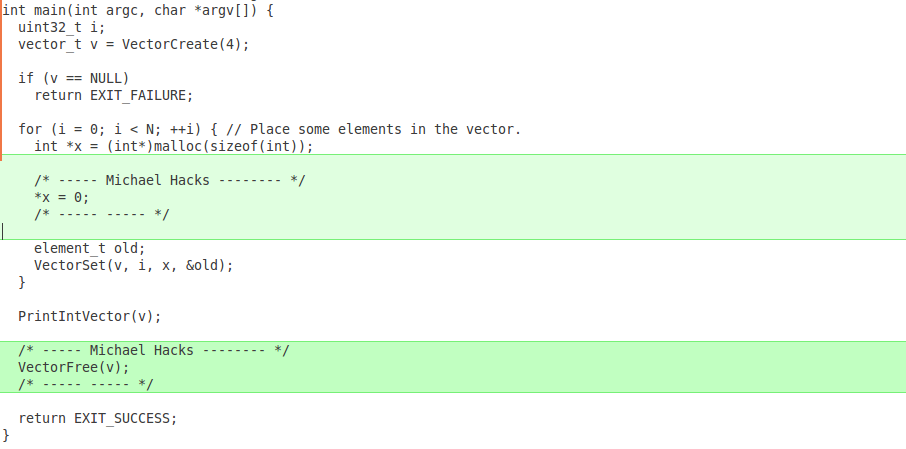
\includegraphics[width=14cm]{modif_exe2_main.png}
\end{center}
\vspace{0.5cm}

Il manquait une initialisation des éléments du vecteur. Les valeurs des vecteurs étaient aléatoires (on lit les dernières valeur dans la RAM). De plus, la fonction de libération du vecteur n'était même pas appelée!\\

La prochaine fonction à améliorer est "VectorCreate" :
\begin{center} 
\hspace{15cm}
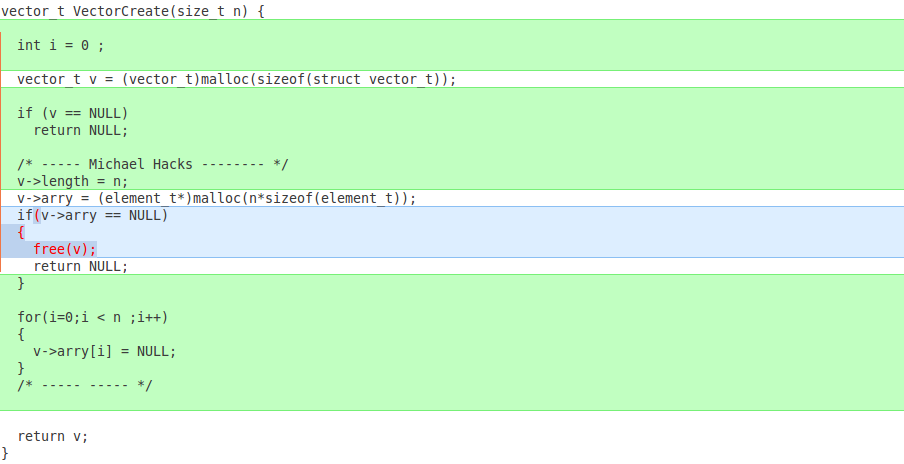
\includegraphics[width=14cm]{modif_exe2_vectorCreate.png}
\end{center}
\vspace{0.5cm}
La mémoire n'était pas libérée en cas de d'erreur d'allocation ultérieure (si l'allocation des éléments échoue, le vecteur alloué juste avant n'était pas libéré) et les éléments n'étaient pas initialisés.
\pagebreak

La modification suivante est l'implémentation de la fonction "VectorFree" qui ne libérait pas une grande partie de la mémoire :
\begin{center} 
\hspace{15cm}
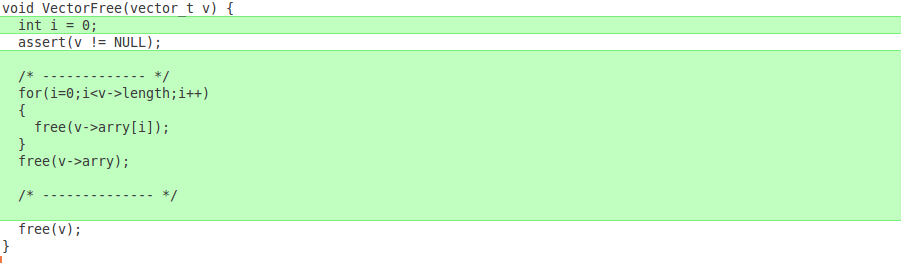
\includegraphics[width=14cm]{modif_exe2_vectorFree.png}
\end{center}
\vspace{0.5cm}
Le programme libérait bien le vecteur, mais pas ses éléments! Donc presque rien n'était libéré.\\

Le dernier gros bug joufflu se trouvait dans la fonction "ResizeArray"  :
\begin{center} 
\hspace{15cm}
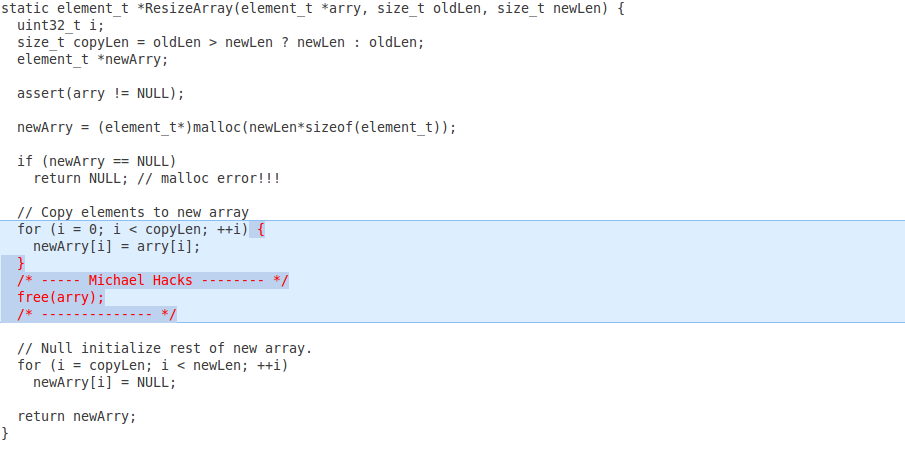
\includegraphics[width=14cm]{modif_exe2_resize.png}
\end{center}
\vspace{0.5cm}
La fonction alloue un nouveau tableau d'une taille "X" et l'initialise avec les valeur du tableau précédent. Par contre, l'ancien tableau n'était pas libéré!

Il restait encore quelques modifications pour initialiser comme il faut les valeurs. 

\pagebreak 
Si on lance cette fois notre outil massif, on voit que la mémoire est libérée correctement : 
\begin{center} 
\hspace{15cm}
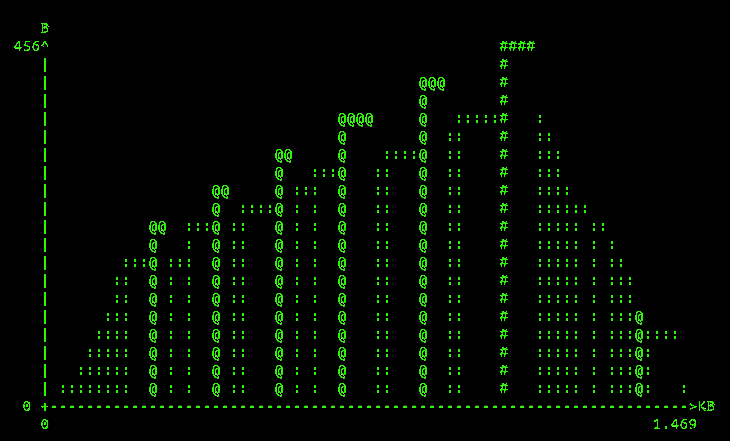
\includegraphics[width=14cm]{massif_apres_exe2.png}
\end{center}
\vspace{0.5cm}

Voici aussi le "memcheck" : 
\begin{center} 
\hspace{15cm}
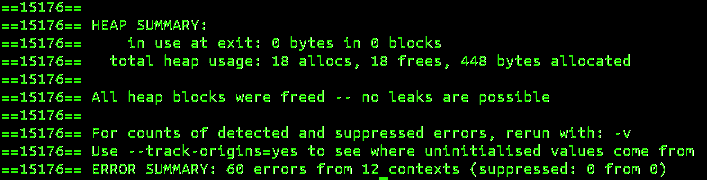
\includegraphics[width=14cm]{memcheck_apres_exe2.png}
\end{center}
\vspace{0.5cm}
On voit que tout à bien été libéré. Il n'existe plus de fuites mémoire. Remarques :  l'outil "Sgcheck" ne donnait pas d'erreur pour ce programme.


